\documentclass{article}
\usepackage[backend=biber]{biblatex}
\usepackage{graphicx}
\addbibresource{refs.bib}
\author{Andrew Pregent}
\date{}
\title{\vspace{-2cm}Midterm Report}
\begin{document}
\maketitle{}
The primary goal set forth by my project proposal was to implement the results of the paper `Volumetric Spot Noise for Procedural 3D Shell Texture Synthesis' by Pavie et al.\cite{pavie:hal-02413269} I am pleased to report that in this I believe I have largely succeeded, though a final task will be to replicate the grass and fur examples they provide, which will require several minor adjustments such as the opaque form of the OI equation and slightly different sampling method for thin Gaussians in the case of the grass example. \\

One of the main difficulties I have encountered in the project thus far has been familiarizing myself with the large area of research which the paper relies on. I have researched and implemented volumetric rendering through slicing, shell texturing, ray marching and EWA splatting, and OI blending techniques. Determining which pieces of each preliminary technique were used by the final results of the paper has also proved to be a challenge in and of itself.

\begin{figure}[h!]
\makebox[\textwidth][c]{
 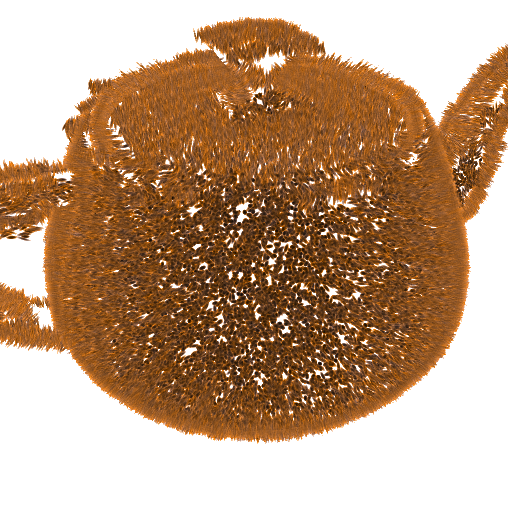
\includegraphics[width=8cm]{figures/hairyteapot}
}
\caption{A teapot with 4440050 Gaussian kernels. The kernel locations still require further work.}
\end{figure}

Once I am satisfied with the fur and grass results I plan to animate the textures, as this seems to be the most realistic of the goals proposed at the start for the time remaining and also seemed to garner the most interest. I also plan to try experimenting with different materials such as bubbles and lichens, and to try blending between distributions.

One additional direction for the project, proposed to me by Dr. Pavie during my correspondence with him, was to use the original EWA splatting formulation with order independent blending. Here he suggests I will need to compute the three dimensional point at which the maximum contribution is reached, though I think this may be specifically for the opaque case. This is something I also wish to explore further, as it would greatly increase the performance of the method as a whole.

\printbibliography

\end{document}
